\documentclass[10pt]{extarticle}
\title{}
\author{}
\date{}
\usepackage[shortlabels]{enumitem}


%paper setup
\usepackage{geometry}
\geometry{letterpaper, portrait, margin=1in}
\usepackage{fancyhdr}
% sans serif font:
\usepackage{cmbright}
%symbols
\usepackage{amsmath}
\usepackage{bigints}
\usepackage{amssymb}
\usepackage{amsthm}
\usepackage{mathtools}
\usepackage{bbold}
\usepackage[hidelinks]{hyperref}
\usepackage{gensymb}
\usepackage{multirow,array}
\usepackage{multicol}

\newtheorem*{remark}{Remark}
\usepackage[T1]{fontenc}
\usepackage[utf8]{inputenc}

%chemistry stuff
%\usepackage[version=4]{mhchem}
%\usepackage{chemfig}

%plotting
\usepackage{pgfplots}
\usepackage{tikz}
\usetikzlibrary{cd}
\tikzset{middleweight/.style={pos = 0.5}}
%\tikzset{weight/.style={pos = 0.5, fill = white}}
%\tikzset{lateweight/.style={pos = 0.75, fill = white}}
%\tikzset{earlyweight/.style={pos = 0.25, fill=white}}

%\usepackage{natbib}

%graphics stuff
\usepackage{graphicx}
\graphicspath{ {./images/} }
%\usepackage[style=numeric, backend=biber]{biblatex} % Use the numeric style for Vancouver
%\addbibresource{the_bibliography.bib}
%code stuff
%when using minted, make sure to add the -shell-escape flag
%you can use lstlisting if you don't want to use minted
%\usepackage{minted}
%\usemintedstyle{pastie}
%\newminted[javacode]{java}{frame=lines,framesep=2mm,linenos=true,fontsize=\footnotesize,tabsize=3,autogobble,}
%\newminted[cppcode]{cpp}{frame=lines,framesep=2mm,linenos=true,fontsize=\footnotesize,tabsize=3,autogobble,}

%\usepackage{listings}
%\usepackage{color}
%\definecolor{dkgreen}{rgb}{0,0.6,0}
%\definecolor{gray}{rgb}{0.5,0.5,0.5}
%\definecolor{mauve}{rgb}{0.58,0,0.82}
%
%\lstset{frame=tb,
%	language=Java,
%	aboveskip=3mm,
%	belowskip=3mm,
%	showstringspaces=false,
%	columns=flexible,
%	basicstyle={\small\ttfamily},
%	numbers=none,
%	numberstyle=\tiny\color{gray},
%	keywordstyle=\color{blue},
%	commentstyle=\color{dkgreen},
%	stringstyle=\color{mauve},
%	breaklines=true,
%	breakatwhitespace=true,
%	tabsize=3
%}
% text + color boxes
%\renewcommand{\mathbf}[1]{\mathbb{#1}}
%\usepackage[most]{tcolorbox}
%\tcbuselibrary{breakable}
%\tcbuselibrary{skins}
%\newtcolorbox{problem}[1]{colback=white,enhanced,title={\small #1},
%          attach boxed title to top center=
%{yshift=-\tcboxedtitleheight/2},
%boxed title style={size=small,colback=black!60!white}, sharp corners, breakable}
%including PDFs
%\usepackage{pdfpages}
\setlength{\parindent}{0pt}
\usepackage{cancel}
\pagestyle{fancy}
\fancyhf{}
\rhead{Avinash Iyer}
\lhead{Economics of Education: Problem Set 3}
\newcommand{\card}{\text{card}}
\newcommand{\ran}{\text{ran}}
\newcommand{\N}{\mathbb{N}}
\newcommand{\Q}{\mathbb{Q}}
\newcommand{\Z}{\mathbb{Z}}
\newcommand{\R}{\mathbb{R}}
\newcommand{\C}{\mathbb{C}}
\newcommand{\iprod}[2]{\left\langle #1,#2\right\rangle}
\newcommand{\norm}[1]{\left\Vert #1\right\Vert}
\setcounter{secnumdepth}{0}
\begin{document}
  \section{Primary School Funding}%
  While listening to the article, I was not particularly shocked at the dynamics of relatively high education spending while also having relatively little to show for it (in the form of amenities for students). The costs of operating a school and paying for teachers is extremely high, especially in the modern era due to the abundance of outside options that educated women have in the labor market. While the Roy model would predict that the higher earnings for college-educated women in outside options would result in lower teacher wages/skill, but there are likely countervailing forces at play that bring the compensation of teachers in relative alignment with the compensation of other college-educated professions, such as increased labor market competition. The result of school funding being relatively confined to the basics of running the school mean that it's likely that fewer field trips/extracurricular activities are funded as the cost of teacher labor and school maintenance increase.
  \section{Student Accountability}%
  \section{Teacher Labor Markets}%
  \begin{enumerate}[(a)]
    \item We see that teacher wage and skill level rise as a result of a higher $\alpha_T$.
      \begin{center}
        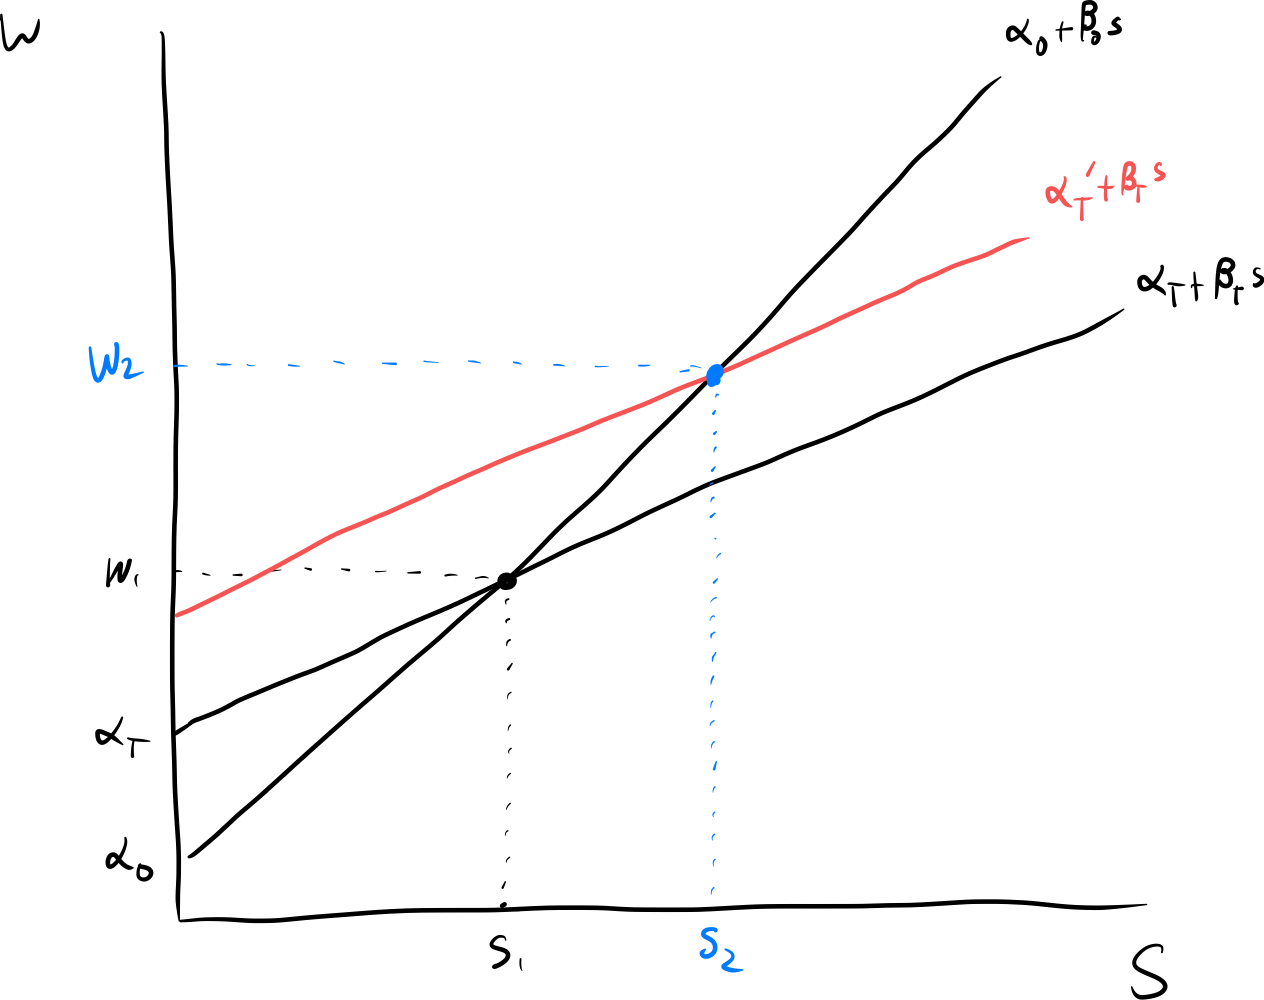
\includegraphics[width=10cm]{images/ps3q3a.png}
      \end{center}
    \item The duty-to-bargain provisions yield lower returns to skill and a flatter wage structure, meaning that the direction of skill and wage changes are ambiguous (in this case, we have drawn a reduction in skill and wage)
      \begin{center}
        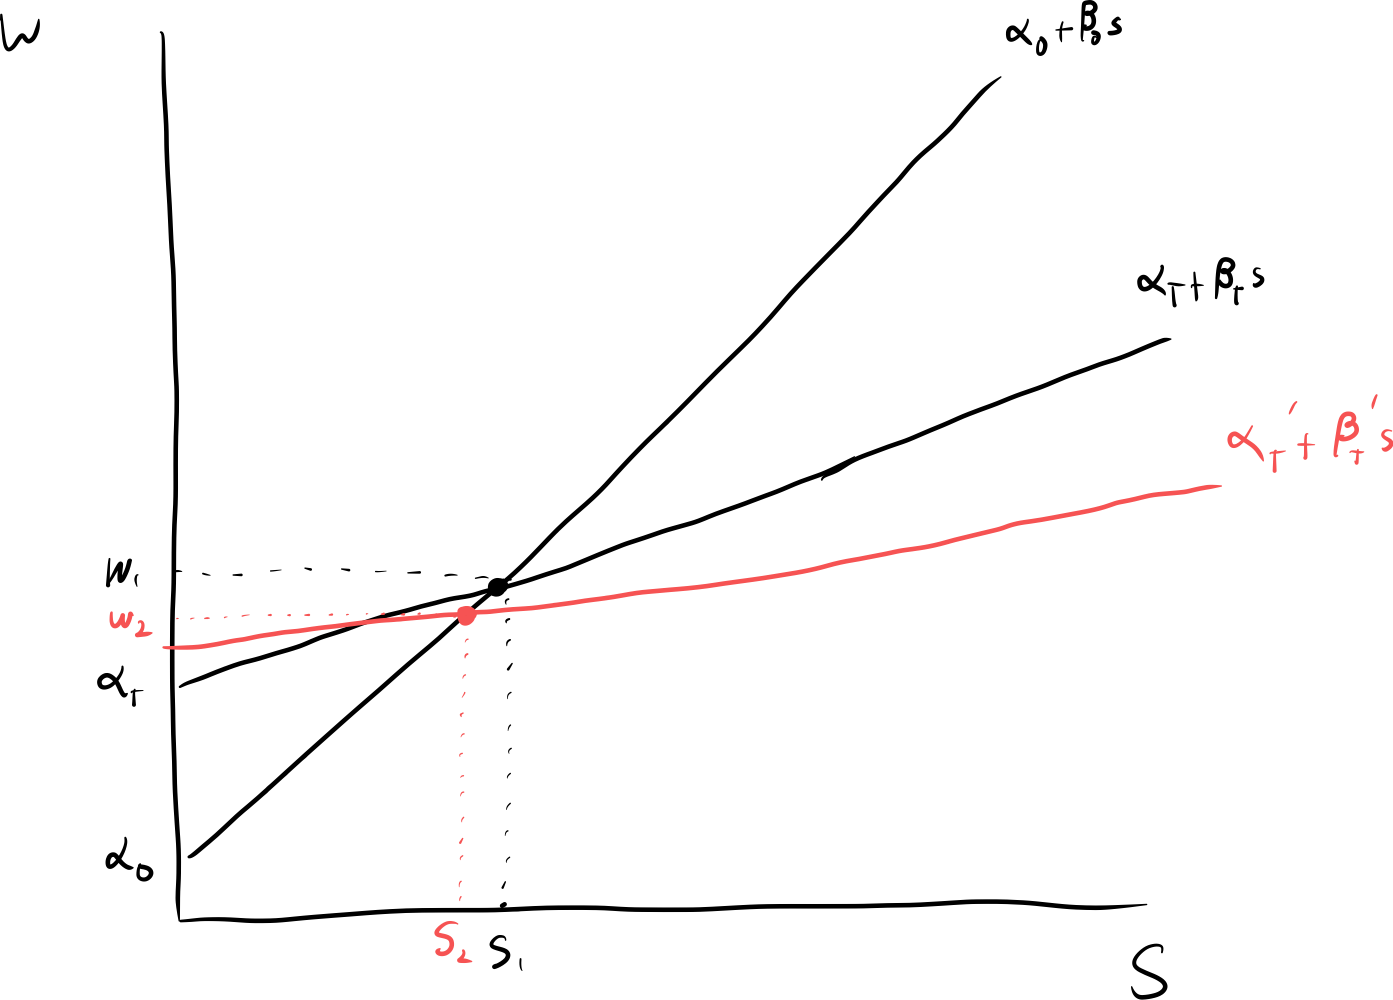
\includegraphics[width=10cm]{images/ps3q3b.png}
      \end{center}
    \item The accountability system increases return to skill, reducing $\alpha_T$ and increasing $\beta_T$.
      \begin{center}
        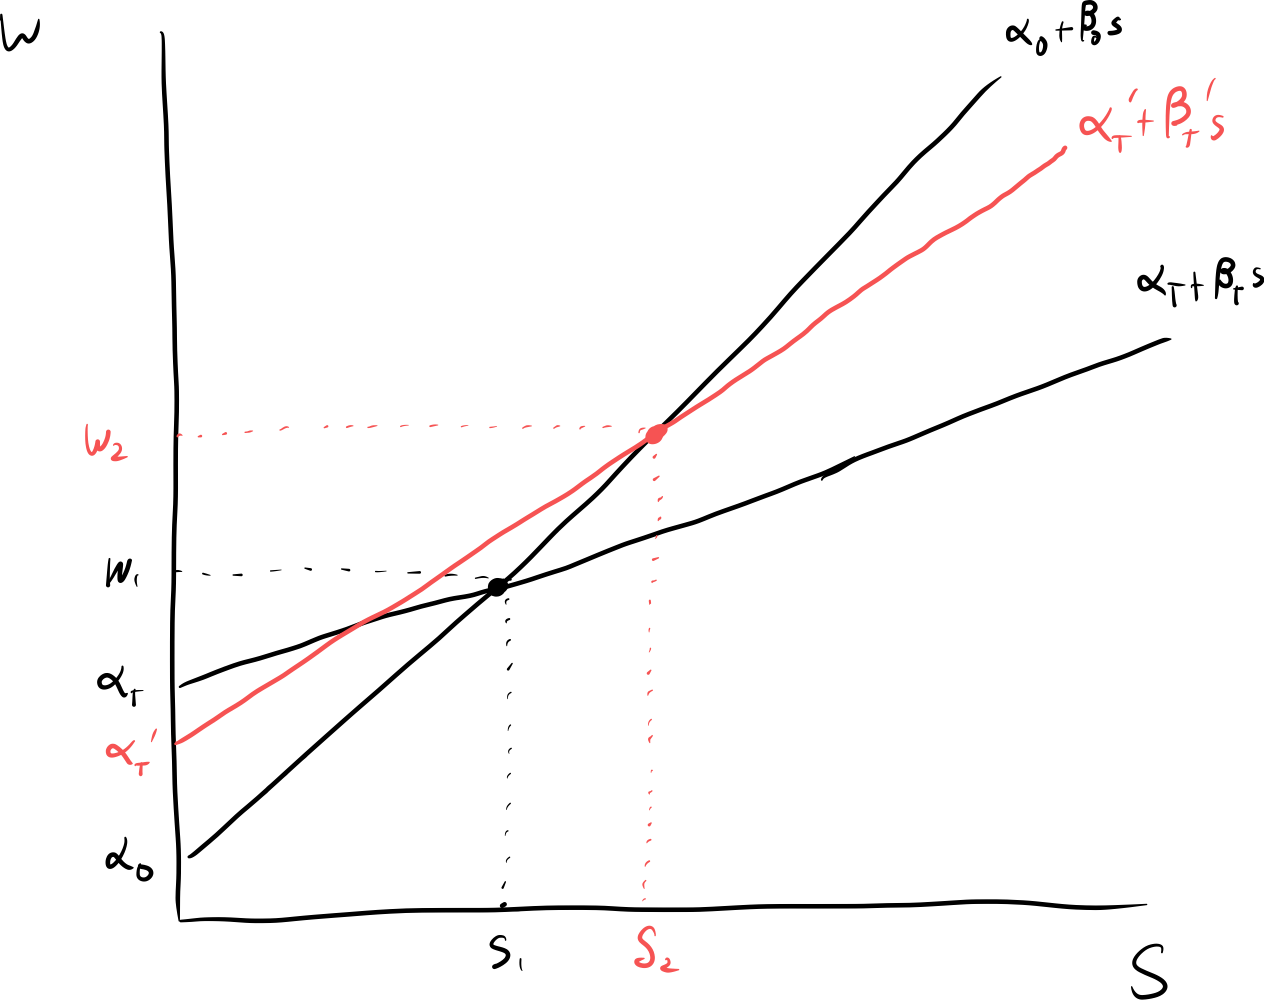
\includegraphics[width=10cm]{images/ps3q3c.png}
      \end{center}
  \end{enumerate}
\end{document}
